\documentclass[11pt]{ltjarticle}
\usepackage[b5paper,bmargin=100pt]{geometry}
\usepackage{luatexja}
\usepackage[utf8]{inputenc}
\usepackage{amsmath}
\usepackage{amssymb}
\usepackage{musicography}
\usepackage{leadsheets}
%\usepackage{luatexja-ruby} 
\usepackage{wrapfig}
\usepackage{caption}
\usepackage{makecell}
\usepackage{graphicx}
\usepackage{xcolor}
\graphicspath{ {./images/} }
\usepackage{hyperref}
\usepackage{subcaption}
\usepackage[document]{ragged2e}

\setchords{
    major-seven = \textsuperscript{M7},
    major-nine = \textsuperscript{M9}
}

\renewcommand*\contentsname{目次}
\renewcommand{\figureautorefname}{図}
\renewcommand{\tableautorefname}{表}
\setlength{\RaggedRightParindent}{\parindent}
\setlength{\abovecaptionskip}{0pt plus 3pt minus 2pt}
\RaggedRight
\pagenumbering{gobble}
\setcounter{tocdepth}{2}

\title{コードオタクが語る東方楽曲分析 \\ \large{第二弾　緋想天 - 砕月からみるメロディーの作り方}}
\author{Metalloid.}
\date{July 2025}

\newcommand{\wc}{\writechord}
\NewDocumentCommand{\sd}{}{\musDegree}
\definecolor{bgc}{RGB}{255, 245, 206}


\begin{document}
%\maketitle

{\huge{コードオタクが語る東方楽曲分析}}
\vspace{3pt}
\hrule
\vspace{3pt}
%\rightline{\large{第二弾　\ruby{緋想天}{SWR} - \ruby{砕月}{Broken Moon}からみるメロディーの作り方}}
\rightline{\large{第二弾　砕月からみるメロディーの作り方}}
\vspace{12pt} \rightline{Metalloid.} \rightline{7/2025}

\tableofcontents

\vspace{12pt}
\hrule

\section{まえがき}
どうも、Metalloid.です。前回はいきなりネクロファンタジアというヘビー級の楽曲を分析したため、内容もかなり難しいものとなっていたと思いますが、今回はもう少しリラックスできるライト回にしようと思い、伊吹萃香のテーマ「砕月」を取り上げることにしました。萃夢想から取り出してくるのが普通かもしれませんが、執筆時現在はちょっとヤンチャな気分なので、敢えて緋想天から引っ張りだすことにしました。\par
前回は某社のw〇rdで文章を打ちましたが、今回は\LaTeX{}を使ってみました。マウス一本で配置ができなくなるために、色々調べ出すことになって、深淵の存在を感知しました。"Lua"がつく名前のものって、なんとなく使っていて安心しますよね。私はもともとコーヒー畑の者ですが。
\section{分析}
\subsection{概要と構成}
今回の曲は、キーが常にC minorで、転調がないです。コード進行も\writechord{Ab} \writechord{Bb} \writechord{Cm} (\writechord{bVI} \writechord{bVII} \writechord{i})をほとんどループしています。また、曲構成は極めて単純で、
\begin{align*}
    \text{\leftrepeat　イントロ$\rightarrow$Aメロ$\rightarrow$サビ$\rightarrow$ポストコーラス$\rightarrow$ソロ回し
　\rightrepeat}
\end{align*}
\begin{wrapfigure}{l}{0.4\textwidth}
    \centering
    \vspace{-20pt}
   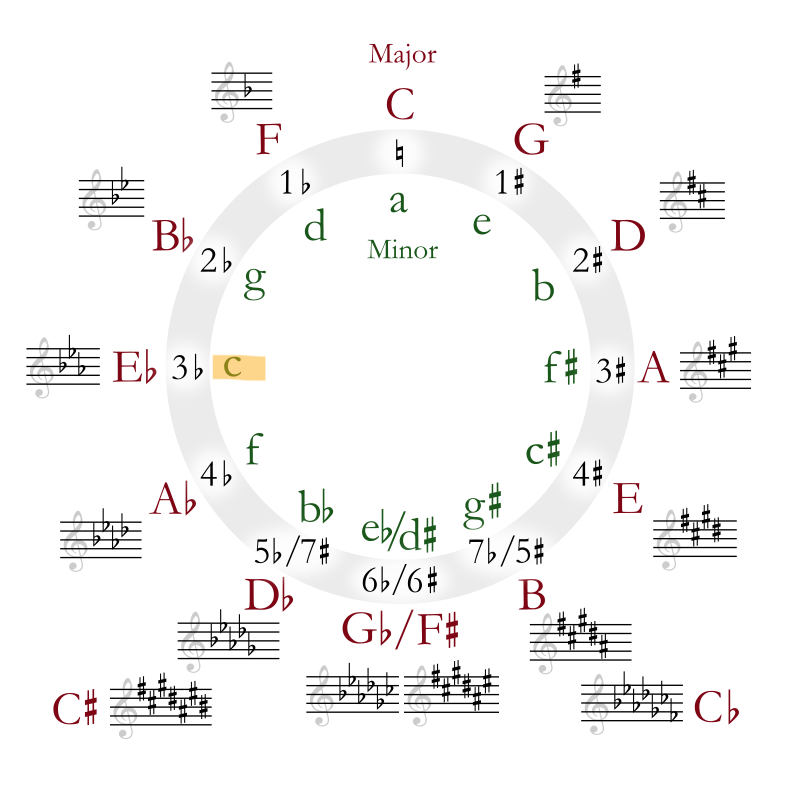
\includegraphics[width=0.4\textwidth]{key overview.png} 
   \label{fig:keyOverview}
   \vspace{-15pt}
    \caption{キー概図\cite{circleFifths}}
\end{wrapfigure}
という形をとっております。セクション分類は独断と偏見で行っていますが、サビを公式音源\cite{OST}40秒目から、ポストコーラスを公式音源1分10秒からと考えています。ポストコーラスという言葉はそもそも聞き慣れないかもしれませんが、実は英語圏におけるセクション分類の言葉の一つで、広くいうと、サビの後に来るセクションであって、サビと似たような性質を継承しながらも、少し相違点のあるものを指します。\cite{wikipediaPostchorus}考えやすい例だと、サビの後に来て、サビの勢いをそのまま保持しつつも、メロディーやコード進行が異なるセクションのことですね。\par
曲の構成自体は結構シンプルなので、今回は和声ではなく、メロディーに注目して分析を進めようと思います。

\subsection{イントロ\&Aメロ}
\begin{figure}[h]
    %\vspace{-50pt}
    
\includegraphics[width=\linewidth]{intro.png}
    \caption{イントロとAメロ一小節}
    \label{fig:intro}
\end{figure}
イントロから、早速癖のあるフレーズが聞こえてきます。このとき、二音目から臨時記号のG\fl(スケール度数でいう\fl \musDegree{5})が現れてきます。
このイントロはそもそも萃夢想版では現れてこないので、このG\fl もこちら限定の仕様となります。このG\fl ですが、曲の中でかなり出てくるので、あらかじめ紹介をしようと思います。これはいわゆる短調ブルースでよく使われるブルーノートという音で\footnote{ブルーノートという言葉は本来微分音の意味合いを持ちますが、多くの場合\fl \sd{5}あるいは\sh \sd{4}で近似されます。}、独特な味や表現力を求めて、通常の短音階から少し外れた音を演奏するというものです。\par
\begin{figure}[t]
    \centering
    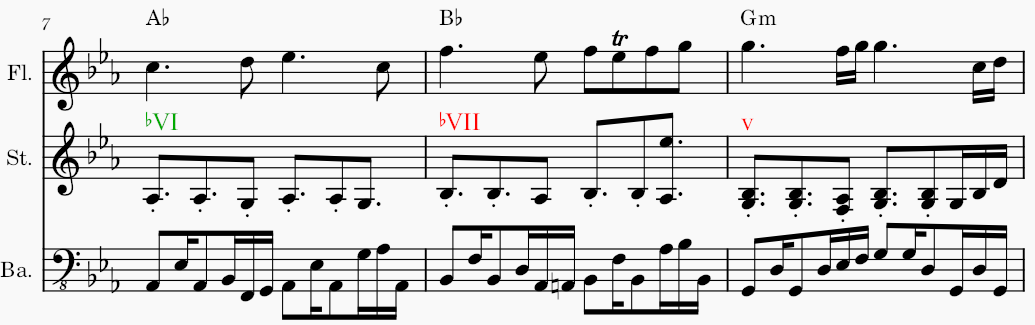
\includegraphics[width=0.9\linewidth]{verse.png}
    \caption{Aメロ（2～4小節抜粋）}
    \label{fig:verse}
\end{figure}
\begin{wrapfigure}[4]{r}{0.5\textwidth}
    \centering
    \vspace{-15pt}
    
\includegraphics[width=\linewidth]{images/verse rhythm.png}
    \caption{Aメロのリズム}
    \label{fig:verseRhythm}
\end{wrapfigure}
さて、Aメロを見ていきましょう。まず、メロディーの大地形をリズムの面から見てみると、\textbf{統一的なリズム}が使用されていることがわかります。(\autoref{fig:verseRhythm}) このような構造をとっていることにより、メロディーに\textbf{一貫性が生まれていて}、多くの人に「ピンと来る」ように感じられるのではないかと思います。音程の面で議論すれば、特徴的なことに、(Aメロだけでなく、曲の各地で)キーの\fl \sd{6}にあたるA\fl が一回も出てきません。\fl \sd{6}は短音階の最も特徴的な音で\footnote{\fl \sd{3}を短音階の最も大切な音とする考え方もありますが、それではドリアン音階(やメロディックマイナースケール)と区別がつかないという問題が起きます。}、よく言えば哀愁を感じさせる、悪く言えば臭い音であるとも言えます。その音を回避することによって、東方のデフォルトたる短音階を使いながらも明るい雰囲気を出すことができます。\par

メロディーの小地形を見ていきましょう。Aメロのメロディーのサンプルとして、最初の三小節を抜粋してきました。(\autoref{fig:verseEscape})まず、E\fl からGに上昇したのち、次の小節の頭のCまで向かいます。
\begin{wrapfigure}[5]{l}{0.4\textwidth}
    \centering
    \vspace{-10pt}
    
\includegraphics[width=\linewidth]{images/verse escape.png}
    \caption{Aメロの小地形}
    \label{fig:verseEscape}
\end{wrapfigure}
ところが、下降中にDについた時点で、フェイントのように一回E\fl にあがってから、飛び降りてCに到達します。このフェイントのような動きはメロディーを華やかにするために用いられる小地形の一つで、\textbf{エスケープ}と呼ばれます。
\autoref{fig:verseEscape}では、エスケープを長方形で囲っています。また、図の通り、エスケープは至る所で使用されていて、一つ目のエスケープが終わってから、次の小節に向かう過程で、再びエスケープが使用されています。ただし、今回はその向きは逆で、最終的にE\fl からFに上昇するために、Cへの下降を挟んでいます。

\begin{figure}[h]
    \centering
   % \vspace{-60pt}
    \fcolorbox{black}{bgc}{
        \begin{minipage}{\linewidth}
        \textbf{エスケープ} \\ ある音から別の音に到達するために、一回逆の方向に進んでから、反転して目的の音に移る修飾。
        \end{minipage}
    }
\end{figure}

\subsection{サビ}
サビのメロディーの特徴として、以下の点が挙げられます：
\begin{enumerate}
    \item 統一的なリズムの使用
    \item ペンタトニックスケールの活用
    \item 笛とペットの間の呼応
\end{enumerate}
順に追っていきましょう。\par
\begin{figure}[h]
    \centering
    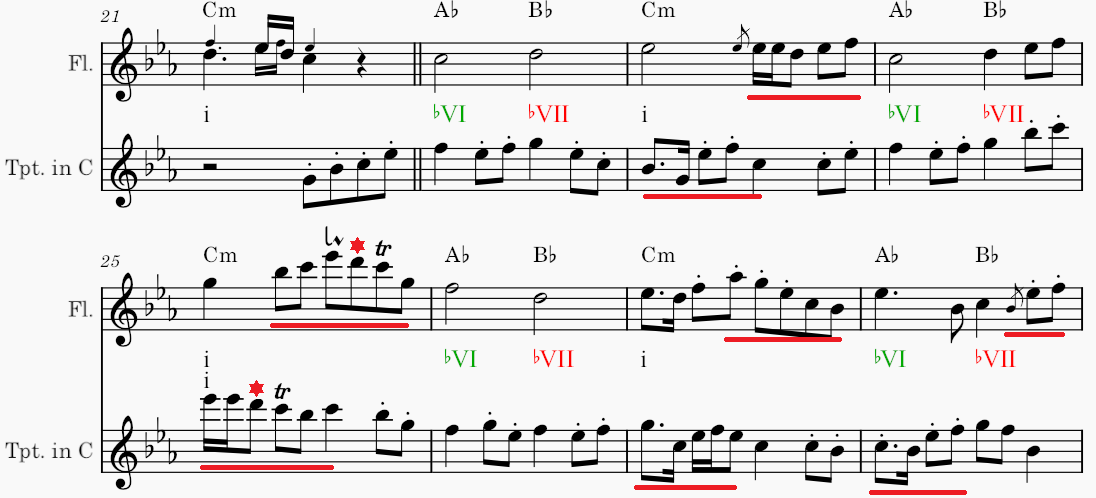
\includegraphics[width=\linewidth]{chorus.png}
    \caption{サビ（管二本のみ表示）}
    \label{fig:chorus}
\end{figure}
まず、リズムに関して、ペットの奏でる主旋律は、Aメロとは異なるリズムでありながら、サビの中では常に大方不変であることがわかります。\par
\begin{wrapfigure}[5]{r}{0.5\textwidth}
    \centering
    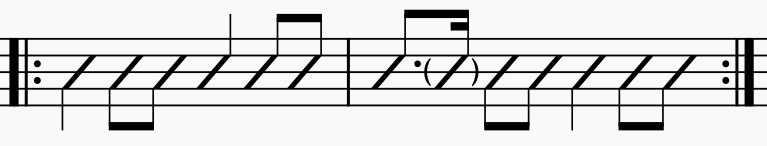
\includegraphics[width=\linewidth]{chorus rhythm.png}
    \caption{サビのリズム}
    \label{fig:chorusRhythm}
\end{wrapfigure}
次に、使っている音ですが、Aメロ同様にA\fl (\fl \sd{6})が見られない上に、D (\sd{2})もほぼ見られず、二回目の\writechord{Cm} (\writechord{i})で経過音として使われているに過ぎません。(\autoref{fig:chorusRhythm}の☆の部分)
つまり、所謂マイナーペンタトニックスケールをほとんど使っているということですね。\textbf{短音階から\sd{2}と\fl \sd{6}を抜いたペンタトニックスケールは非常に安定していて、そこから適当に音を選んでつなぎ合わせても、一言でいう「カッコイイ」フレーズが出来上がります。}

\begin{figure}
    \centering
    \vspace{-60pt}
    \fcolorbox{black}{bgc}{
        \begin{minipage}{\linewidth}
            \textbf{メジャー・マイナーペンタトニックスケール} \\
            \vspace{5pt}
            \begin{wrapfigure}{r}{0.3\linewidth}
                \centering
                \vspace{-35pt}
                
\includegraphics[width=\linewidth]{images/major pentatonic.png}
                
\includegraphics[width=\linewidth]{images/minor pentatonic scale.png}
                \caption{諸Cペンタトニックスケール}
                \label{fig:pentatonic}
            \end{wrapfigure}
            それぞれ長音階、短音階からそれぞれの「不安定」「臭い」「癖強い」音を除去して使いやすくした音階。長音階から\sd{4}, \sd{7}、短音階からは\sd{2}, \fl \sd{6}が除去される。それぞれヨナ抜き（長）音階、ニロ抜き（短）音階とも。癖がない分、よく言えば何にでも合う、悪く言えば感情が乏しい。
            \vspace{10pt}
        \end{minipage}
    }
\end{figure}
東方原作タイトルテーマで毎度お馴染の「いつものフレーズ」も、実はペンタトニックスケールを活用した一例ですね。\par
続けて、このサビに限らず曲の最大の特徴として、笛とペットが同時に鳴っている点があります。これも、緋想天版限定の特典ですね。とはいえ、闇雲に重なっているわけではなく、ペットと笛の間でしっかりとした\textbf{コールアンドレスポンス}が成り立っている：\autoref{fig:chorus}を見ていくと、ペットが光るフレーズを演奏した後、その「投げられた問い」に対して同小節の後半で必ず笛が応答して、部分的に一致するフレーズを吹いています。しかも、片方が光っている間、もう片方は伸ばし等、あまり目立たないフレーズを演奏しています。こうして見ると、サビの入りでペットが登場するときに笛が一旦去るのは計算されていると云えますね。\par
それでは再び主旋律の小構造を見ていきましょう。
\begin{figure}[h]
    \centering
    
\includegraphics[width=\linewidth]{images/chorus contour.png}
    \caption{サビの輪郭}
    \label{fig:chorusContour}
\end{figure}
音を採ってみると、メロディーは前述の統一的リズムに則って微小な上り坂と下り坂を繰り返していることがわかります。(\autoref{fig:chorusContour})言い変えると、\textbf{基礎的な構成単位「三音の上り坂」を、色んな形へと変化発展させながらサビを作り上げている}ということです（「下り坂」は「上り坂」を反転させて得られるので）。楽譜を俯瞰すると、坂道の配置の仕方も、二小節周期の単位を四単位使って「起承転結」を作っていることも見えてきます。特に面白いのは、最初の二回（「起」「承」）で、\writechord{Ab}が鳴っているときは必ず坂の方向が「上向き」になっているところですね。\writechord{Ab} (\writechord{bVI})はキーにおいてサブドミナントの役割を持ったコードで、コード進行においては、勢いを作る、助走の役割を担っています。まさしく上り坂を登るにふさわしいコードに思えてしまいますね。逆に、落ち着きを表すトニックの役割をもつ\writechord{Cm} (\writechord{i})に対しては、下り坂がチョイスされているのもおもしろいですね。ところが、「転」にあたる三回目では、\writechord{Ab}に対して下り坂を使っていて、バリエーションを出し、「結」の部分では、すべてを統合した「丘」型の輪郭が現れます。これがすべて一つの「坂道」の変化発展として生み出された（であろう）と考えると、意外と面白いですね。\par
最後に、この「坂道」が小節の頭から始まるのではなく、強調される最後の音が小節の頭に来ているのも基本的な工夫ですね。そうすることによって、小節の頭に到達する前の\textbf{「摑み」の小地形}を発生させることができるからです。
\subsection{ポストコーラス}
ポストコーラスに関して云えば、もう予想はついていると思いますが、\autoref{fig:post-chorus}, \autoref{fig:post-chorusRhythm}で見えるように、再び\textbf{「コーレス」}と\textbf{「統一的なリズム」}が現れます。
\begin{figure}[h]
    \centering
    
\includegraphics[width=\linewidth]{images/post-chorus.png}
    \caption{ポストコーラス}
    \label{fig:post-chorus}
\end{figure}
\begin{wrapfigure}[5]{l}{0.4\textwidth}
    \centering
    
\includegraphics[width=\linewidth]{images/post-chorus rhythm.png}
    \caption{ポストコーラスのリズム}
    \label{fig:post-chorusRhythm}
\end{wrapfigure}さて、再びズームインしてみましょう。(\autoref{fig:post-chorusContour})メロディー全体の輪郭として、サビの間の坂の形に対して、今回は「波」の形が描かれています。サビ同様、同じ「波」の形が起承転結を成しているようで、二回目の波は一回目の波を下にずらしたもので、三回目は波を崩していてまさしく「転」の箇所であると云えます。「結」の部分では波が反転されていますね。また、セクションの終わりの方で、\textbf{サビの最後のフレーズとほぼ同一のフレーズ}が用いられています。悪く言うと焼き直しですが、良くいうと一貫性のある執筆です。メロディーを作るにあたってそれなりの\textbf{一貫性があるのは馴染みやすさを生む}ので、教科書的と評価することもできます。\par
さて、ここで本日紹介したい三つ目のメロディー小地形があります。
\begin{figure}[h]
    \centering
    
\includegraphics[width=\linewidth]{images/post-chorus contour.png}
    \caption{ポストコーラスの輪郭}
    \label{fig:post-chorusContour}
\end{figure}
\autoref{fig:post-chorusContour}で長方形で囲っている箇所に注目しましょう。一つ目の例では、\musEighth のDとB\fl が、次の強拍に位置するCを「囲って」います。これは\textbf{エンクロージャー}という小地形で、度々メロディーライティングの中で用いられるテクニックです。続いて二つ目の長方形では、修飾音を無視すると、Gの音を導き出すために、その前段階でFとB\fl が演奏されています。これもエンクロージャーです。
\begin{figure}[h]
    \centering
   % \vspace{-60pt}
    \fcolorbox{black}{bgc}{
        \begin{minipage}{\linewidth}
        \textbf{エンクロージャー} \\ 目当ての音程に辿り着くために、その上・下の音程を踏んでおくメロディーテク。半音で囲う場合(chromatic enclosure)も、スケールトーンで囲う場合(diatonic enclosure)もある。
        \end{minipage}
    }
\end{figure}
\subsection{ボーナス| ソロ}
萃夢想版と緋想天版の大きな違いとして、最後のペットと笛のソロバトルがあります。ここでは「メロディー」というよりかは「ソロフレーズ」が用いられているので、本稿の趣旨からは少しそれますが、折角なので少し見てみることにします。\par
譜起こしをせずとも、ペットソロは既存のメロディーを崩していることは感じられると思います。いざ見てみると、リズムの変更はありますが、\textbf{メロディーの音}（色付き）\textbf{は再利用されていました}。
\begin{figure}[h]
    \centering
    
\includegraphics[width=\linewidth]{images/solo trumpet.png}
    \caption{ペットソロ三小節}
    \label{fig:soloTrumpet}
\end{figure}
ペットから笛への受け渡し部分は教科書的で、笛がペットと同じ音を鳴らして、ペットが撤退することによって受け渡しが成就します。\par
\begin{figure}[h]
    \centering
    
\includegraphics[width=\linewidth]{images/solo transition.png}
    \caption{ソロ受け渡し部分}
    \label{fig:soloTransition}
\end{figure}
\begin{figure}[h]
    \centering
    
\includegraphics[width=\linewidth]{images/solo flute.png}
    \caption{笛ソロ残り}
    \label{fig:soloFlute}
\end{figure}
このソロで多くの臨時記号が出てきますが、その半分はイントロのところで顔をみせたブルースからの\fl \sd{5}です。残るE\na も実は、黒人音楽やロックのブルーノートの一種で、短調でマイナーペンタトニックや、そこから作られるブルース音階だけではなく、バリエーションとしてメジャーペンタトニックを使ってみることによって\na \sd{3}が発生するというパターンです。
\begin{figure}[h]
    \centering
    \fcolorbox{black}{bgc}{
        \begin{minipage}{\linewidth}
            \textbf{メジャー・マイナーブルーススケール} \\
            \begin{wrapfigure}{r}{0.28\linewidth}
                \centering
                \vspace{-35pt}
                
\includegraphics[width=\linewidth]{images/blues scale.png}
                \caption{諸C六音ブルーススケール}
                \label{fig:blues}
            \end{wrapfigure}
            ペンタトニックスケールにそれぞれ最も頻繁に使われるブルーノート（の平均律近似）を追加した音階。ブルーノートは多種あるので、ブルース音階も厳密には多種ある。この六音音階はその中で代表的なもので、メジャーペンタトニックに\fl \sd{3}、マイナーペンタトニックに\fl \sd{5}を追加することで得られる。
        \end{minipage}
    }
\end{figure}
\subsection{まとめ}
今回は難しい和声的概念から一旦離れ、緋想天 - 砕月を通して、メロディーの構成について深堀りしてみました。
メロディーには多段階での構造があり、砕月の例では、
\begin{itemize}
    \item 大きな構造として
    \begin{itemize}
        \item リズムの再利用
        \item 起承転結
        \item 癖の出にくいペンタトニックスケールの活用
    \end{itemize}
    \item 小さな構造として
    \begin{itemize}
        \item エスケープ
        \item エンクロージャー
        \item 楽器間のコーレス
    \end{itemize}
\end{itemize}
が存在することを見ていきました。
大きな構造はメロディーに一貫性やわかりやすさを与え、小さな構造はメロディーに味を与えたり、メロディーを書きやすくします。\par 
さらに、この曲では同じフレーズを少しずつ変化させながら再利用していく手法も用いられているのではないかと考察しました。これを行うことにより、リズムの再利用と同様、一貫性や親しみやすさが生まれるだけでなく、書き手からしてもメロディーが書きやすいのではないかと思います。もし読者の皆様にメロディーを書く日が訪れたならば、是非実践してみてください。
\section{付録}
\subsection{音楽理論基礎 (再掲)}
以下は基本的に前回の付録にマイナーチェンジを施したものです。\par 
執筆途中の段階で、音楽を知っている方でも、音楽理論をしらないとこの文章を読んでいても何も楽しくもないのだろうなと気づき始めたので、“ダイジェスト版“で基本的な音楽理論の概念を付録に載せようと思い至りました。といっても、簡潔な文章を書くのが苦手なので、本当にダイジェストになるかはわかりません。ごめんなさい。
\subsubsection{半音階}
ピアノや鍵盤をみたことがある人ならわかると思いますが、一オクターブの中には12個の音があります。ソルフェージュではこれらをド, ド\sh /レ\fl , レ, レ\sh /ミ\fl , ミ, ファ, ファ\sh /ソ\fl , ソ, ソ\sh /ラ\fl, ラ, ラ\sh /シ\fl , シと呼びますが、僕はブリティッシュインペリアリズムに負けた人なので、これらをC, C\sh /D\fl , D, D\sh /E\fl , E, F, F\sh /G\fl, G, G\sh /A\fl , A, A\sh /B\fl , Bと呼びます。特別に和な心持でこれを読まれている方はきっと心の中ではハ, 嬰ハ/変ニ, ニ, 嬰ニ/変ホ, ホ, ヘ, 嬰ヘ/変ト,ト, 嬰ト/変イ, イ, 嬰イ/変ロ, ロと呼んでいるのでしょう。若かりし4.5年前の自分の抱いた疑問にて、B\sh とE\sh , C\fl とF\fl は一体どこにいったのだ、という問いがありましたが、これはピアノの鍵盤をみたらわかります。E\sh =Fなのです。\textbf{ただし、これは近代的なチューニング体系を用いる音楽に限られ、本来C\sh とD\fl は異なる音、B\sh とCも異なる音であると考えられていました。}半音階で隣接した二つの音の差を半音、二半音の差を全音と呼びます。つまり半音は世に出くわすほとんどの音楽においてはピッチの距離の最小単位となります。
\subsubsection{音程}
音程をピッチの同義語だとよく思われますが、厳密にはそれは嘘で、辞書的には「二つの音のピッチの距離」を意味します。音程の言葉の例としては「完全五度」「長六度」「短三度」などがあり、何かしらの「質」と「数」が組み合わさっています。音程の「数」は二つの音の間にまたぐアルファベット種の数、楽譜上での線（と空白）の数、あるいは鍵盤上の跨ぐ白鍵の数と認識すると良いでしょう。ただし、1から数えられます。\par
例：
\begin{itemize}
    \item \textbf{A}と\textbf{C}はA, B, Cの三文字を跨ぐので、\textbf{三度}の距離があります
    \item \textbf{F}\sh と\textbf{D}\sh はF, G, A, B, C, Dの六文字を跨ぐので、\textbf{六度}の距離があると云えます
\end{itemize}\par
しかし、このままでは問題があります。例えば、CとEとの間の音程は三度であるといえます。同様に、DとFの間も三度の差があります。しかし、それぞれの距離を半音ベースで数えると（0から数えて）CとEは四半音差、DとFは三半音差です。つまり、音程の「数」では実際の音の距離を一意的に決定・記述することができないのです。そのために、音程の言葉には「質」が接頭辞としてつきます。これは「長」「短」「増」「減」「完全」の五種あり、
\begin{enumerate}
    \item 歴史的経緯から(ユニゾン(0半音)、オクターブ(12半音))、7半音の「五度」、5半音の「四度」には「完全」がつきます。（ただ、六半音の音程については別名の「トライトーン」が存在します）
    \item それ以外では、白鍵だけを考えたときに総当たりを行い、「デカい」に「長」、「小さい方」に「短」がつきます。
    \item 上のスキームに当てはまらなかったものに対して、「減」と「増」がつきます：
    \begin{itemize}
        \item 完音程や長音程を一半音広めるときに「増」
        \item 完音程や短音程を一半音狭めるときに「減」
    \end{itemize}
\end{enumerate}
いきなりルールを説明されても難しいと思うので、実例をみてみましょう。
\begin{itemize}
    \item \textbf{A}と\textbf{G}の間は、A B C D E F Gの七種の文字が存在し、半音距離は10なので、\autoref{tab:intervals}を以て短七度の距離であるといえる
    \item \textbf{A}と\textbf{F}\sh の間では、A B C D E Fの六種の文字が存在し、半音距離は9なので、長六度の距離である
    \item \textbf{A}と\textbf{E}の間は、A B C D Eの五種の文字が存在し、半音距離は7なので、\autoref{tab:intervals}を以て完全五度の距離であるといえる
    \item \textbf{A}と\textbf{E}\fl の間では、A B C D Eの五種の文字が存在するが、半音距離は6であるので、上記の完全五度を狭めたものであるとして、減五度(\autoref{fig:intervals}参照)であると云える。また、この場合は慣用名のトライトーンという言葉も使うことができる。
    \item \textbf{A}と\textbf{D}の間では、A B C Dの四種の文字が存在し、半音距離は5なので、完全五度の距離である
    \item \textbf{A}と\textbf{D}\sh の間では、A B C Dの四種の文字が存在するが、半音距離は6であるので、上記の完全四度を広めたものであるとして、減五度(\autoref{fig:intervals}参照)であると云える。また、この場合は慣用名のトライトーンという言葉も使うことができる。
    \item \textbf{A}と\textbf{G}\fl の間では、A B C D E F Gの七種の文字が存在するが、半音距離は9であるので、上記の短七度を狭めたものであるとして、減七度(\autoref{fig:intervals}参照)であると云える。（G\fl はF\sh と「同じ」であるとして、長六度として丸めてしまいたいと思うかもしれないが、命名のルールと、冒頭で述べたようにそもそもF\sh とG\fl という音符が同じピッチを指すとは限らないことから、長六度という名前は原理的には不適切である。）
\end{itemize}
\begin{figure}
    \begin{subfigure}{0.4\textwidth}
        \centering
        
\includegraphics[width=1\linewidth]{images/intervals.png}
        \caption{音程例}
        \label{fig:intervals}
    \end{subfigure}
    \begin{subfigure}{0.5\textwidth}
        \centering
        
\includegraphics[width=1\linewidth]{images/interval quality.png}
        \caption{音程の質}
        \label{fig:音程の質}
    \end{subfigure}
    \centering
    \caption{音程について}
\end{figure}
\begin{table}
    \centering
    \caption{基本的音程名}
    \begin{tabular}{|c|c|c|c|}\hline
        半音距離 & 和名 & 英名 & 略\\ \hline
        0 & ユニゾン &  (Perfect) Unison& P1\\
        1 & 短二度 &  Minor Second& m2\\
        2 & 長二度 &  Major Second& M2\\
        3 & 短三度 &  Minor Third& m3\\
        4 & 長三度 &  Major Third& M3\\
        5 & 完全四度 &  Perfect Fourth& P4\\
        6 & トライトーン&  Tritone& TT\\
        7 &  完全五度 &  Perfect Fifth& P5\\
        8 &  短六度 &  Minor Sixth& m6\\
        9 &  長六度 &  Major Sixth& M6\\
        10 & 短七度 &  Minor Seventh& m7\\
        11 &  長七度 &  Major Seventh& M7\\
        12 &  オクターブ &  (Perfect) Octave& P8\\\hline
    \end{tabular}
    \label{tab:intervals}
\end{table}
覚えることが大変かもしれませんが、これだけ押さえておけば基本的にはあとあともう困らないと思います。
\subsubsection{コード}
コードというのは最も基本的な理解ではある音（ルート）の上に三度を順番に積み重ねて作るものです。では色々組み合わせて作っていきましょう。三度の種類は二種類あったので、音を三つ使ったコードは4パターンありえます。（\autoref{fig:triads}）コードの命名は、ルートの上に何がくるかによって決定されます。例えば、右から二つ目はルートの上にM3とP5を載せたときに生まれるもので、メジャーコードと言います。長調の響きがする明るい子です。逆に、左から二番目はルートの上にm3とP5を載せたもので、マイナーコードといい、暗めの響きがします。左端のものは、ルートの上にm3とTT(or減五度)を載せたもので、ディミニッシュコードと呼ばれ、鬱な響きを持ちます。最後に右端はM3とA5をルートの上に重ねたもので、オーグメンティッドコードといい、不安定な響きを持ちます。\par
続いて、三つの音ではなく、それを拡張して四つの音を用いてコードを作ってみましょう。（\autoref{fig:seventhChords}）これらは、四つ目の音がルートからみて七度にあたることになるので、大きくセブンスコードと呼ばれます。真ん中の例はメジャーコードの上にm7を載せたもので、ドミナントセブンスコードと呼ばれます。その右にはメジャーコードにM7をのせたもので、メジャーセブンスコード、左はマイナーコードにm7をのせたものでマイナーセブンスコードと呼ばれます。左端のものはディミニッシュコードにm7を付けたもので、マイナーセブンスフラット5や、ハーフディミニッシュセブンスと呼ばれます。右端はルートの上に短三度、減五度、減七度がついたものであり、ディミニッシュセブンスコードと呼ばれます。ほとんどの場合、別のドミナントセブンスコードのルートだけを半音上げるという動作によって曲の中で出現します。(\writechord{C7} \rightarrow \writechord{C#dim7})
\begin{figure}
    \begin{subfigure}{0.4\textwidth}
        \centering
        
\includegraphics[width=1\linewidth]{images/triads.png}
        \caption{簡単なコード}
        \label{fig:triads}
    \end{subfigure}
    \begin{subfigure}{0.5\textwidth}
        \centering
        
\includegraphics[width=1\linewidth]{images/seventh chords.png}
        \caption{セブンスコード}
        \label{fig:seventhChords}
    \end{subfigure}
\centering

\end{figure}
\subsubsection{調・キー}
20世紀までの近代西洋音楽では、半音階のすべての音を使わず、同時に使うのは大体そこから七個だけを選んだ部分集合です。この部分集合を調、スケール、音階、あるいはキーと呼びます。簡単に云うと、絵画でいう「パレット」のようなものです。調には一つ基準点として機能する「トニック」が存在し、そこから音程を用いてスケールを定義できます。最も有名なスケールはメジャースケール（長調）で、トニックのM2, M3, P4, P5, M6, M7上の音をチョイスしてパレットが構成されます。ドを基準にしてとっていくと、つまりドレミファソラシ (C, D, E, F, G, A, B)ですね。他にも、東方をやる上では必須な、自然短音階(ナチュラルマイナースケール、natural minor scale)というものもあります。こちらはトニックからM2, m3, P4, P5, m6, m7上の音を選んだものです。Cを基準にして具体的に書いていくと、Cマイナースケール≡C D E\fl , F, G, A\fl , B\fl となります。そして、よくみるものに和声短音階(ハーモニックマイナースケール、harmonic minor scale) というものもあります。こちらはR, M2, m3, P4, P5, m6, M7の構成で、C基準でいくとC D E\fl , F, G, A\fl , B\na です。命名や用途は書き出すと長く語ってしまうので興味のある方は調べてみてください。\par 
キーの中の音を、トニックからの音程をベースに数字を与え、記述することができます。例えば、C majorにおいて、Aは六度目なので\sd{6} と書き表すことができ、C minorで、Fは四度目なので\sd{4}, A\fl は六度目なので\fl \sd{6}と表記することができます（調を明らかにできるように\sd{6}ではなく\sd{b6}と書きました。詳細は付録末にて）。これによって、絶対音感を持たない身分であるせいで、キーが不明であっても、聞こえる音を認識し、記述することができます（例えば、「あ、今\na \sd{7} \sd{2} \sd{1}という旋律が聞こえたな。」と）\par
また、キーという「パレット」に存在しない音を例外的に採用することが存在し、それはよく「臨時記号」と呼ばれます。臨時記号は特異的な雰囲気を纏うことが多く、音楽的な意味が大きく込められていることが多いので、度々分析の対象となります。\par
キーを楽譜上に表すのが「調号」で、これは\trebleclef \bassclef のすぐ右に書かれる\sh や\fl の集まりです。これらは、キーを設定するために選ばれた音の\sh や\fl を因数分解のように「外に括りだして」楽譜を読みやすくするものです。逆に、臨時記号は楽譜途中の\sh や\fl であり、これらは一小節が終わるとリセットされると思って読むと良いでしょう。
\subsubsection{コードの機能}
キーというパレットを定めたうえで、その音を使ってコードというのをつくってみると、例えば、C majorから選んでいくと、C, D, E, F, G, A, Bという音が許されるので、そこから作られるコードは\writechord{C, Dm, Em, F, G, Am, Bdim}となります。逆にC minorから音を選んでつくると、\writechord{Cm, Ddim, Eb, Fm, Gm, Ab, Bb}のコードを作ることができます。こうしてキーの中の音を使って作ったコードをダイアトニックコードと呼びます。ダイアトニックコードは、キーの中ではある特定の雰囲気・役割を持つという基本的な考え方（機能和声という考え方）があり、その理論のもとでは、コードの役割は大きく分けて三つに分類されます：
\begin{itemize}
    \item トニック：安定した響きを持つコードです。イメージでいうと、曲の終わりや、お辞儀の最後です。
    \item ドミナント：不安定な響きを持ち、トニックが次に来ると快楽を覚えさせるコード。ドミナントからトニックコードに向かうことを「解決」と呼びます
    \item サブドミナント（プレドミナント）：トニックに対する解決力は弱いが、ドミナントを持ってくるための下準備・勢い作りを
することができる。癖が強いコードが多い。
\end{itemize}
どのダイアトニックコードがどのような役割を持つのかは付録の最後に説明しています。\par
このコードの役割を理解すると、コード進行は一つの物語を作ることが想像できます。トニックから始まり、サブドミナントで勢いを作り、ドミナントで緊張を作ってトニックに解決するというサイクルは、「起承転結」の音楽版であると云えます。
\subsubsection{ローマ数字表記}
スケールにおける帽子付き数字（スケール度数）と同様に、コードをキーの中での役割によって記述する方法があります。それは、コードのルートのスケール度数を記述することです。これは、コードのキーの中での聞こえ方・役割が、ルートのスケール度数に大方依存するという経験則的大筋から由来します。逆に、同じコードでも、異なる文脈（キー）の中で演奏すれば、その意味や聞こえ方は変わってくるということです。例えば、キーC minorで演奏する\writechord{Gm}はドミナントコードですが、キーD minorで演奏する\writechord{Gm}はサブドミナントであり、全く雰囲気が違います。スケール度数と同様に、ローマ数字を用いることによって、キーを併記しないでコード進行を記述し、記述を一般化することができます。例えば、東方原曲での数多くの曲は「\writechord{bVI bVII i}」（例：キーC minorにおける\writechord{Ab} \wc{Bb} \wc{Cm}, キーD minorにおける \writechord{Bb} \writechord{C Dm}）というコード進行を使っているという事実があります。ローマ数字の振り方は付録の最後にて説明しています。
\subsection{本稿における表記法と思想}
音楽理論を扱う世のマテリアルでは表記（と流派）が異なることも多いので、本稿で使用する表記とコードの解釈について追記します。特に、東方は短調ベースで書かれることが多く、臨時記号も多用するので、それに適応した表記として、長調としての表記・分析より短調としての表記や分析を行うことが多いと思います。\par
具体的に、コードのルートに対する度数とスケ
ールに対する度数を区別するため、後者をアクセント
付きの数字で表記していきます。（\autoref{fig:scales}）\par
\begin{itemize}
    \item  長音階に関しては \sd{1} \sd{2} \sd{3} \sd{4} \sd{5} \sd{6} \sd{7} と表記
    \item 自然短音階は \sd{1} \sd{2} \fl \sd{3} \sd{4} \sd{5} \fl \sd{6} \fl \sd{7} と表記
    \item その上で、臨時記号をその都度用いる（例: 和声短音階は \sd{1} \sd{2} \fl \sd{3} \sd{4} \sd{5} \fl \sd{6} \na \sd{7} ）
\end{itemize}

\begin{figure}
    \centering
    \begin{subfigure}{0.4\textwidth}
        \centering
        
\includegraphics[width=\linewidth]{images/major scale.png}
        
\includegraphics[width=\linewidth]{images/minor scale.png}
        \caption{長音階、短音階}
        \label{fig:scales}
    \end{subfigure}
    \begin{subfigure}{0.4\textwidth}
        \centering
        
\includegraphics[width=\linewidth]{images/major scale chords.png}
        
\includegraphics[width=\linewidth]{images/minor scale chords.png}
        \caption{長音階、短音階のダイアトニックコード}
        \label{fig:diatonicChords}  
    \end{subfigure}
    \caption{本稿での表記}
    \label{fig:notation}
\end{figure}

また、コードのローマ数字表記に関して、メジャーコードとマイナーコードの表記法を区別します。（\autoref{fig:diatonicChords}）
\begin{itemize}
    \item メジャーコードは大文字
    \item マイナーコードは小文字
    \item コードエクステは重要であると判断した場合に表記
\end{itemize}
続いてダイアトニックコードの役割ですが、ダイアトニックコードの役割は教材・ソースによって割れることも多々あるので予めここで本稿においての考えを断っておきます。（\autoref{tab:diatonicFunctions}）
\begin{itemize}
    \item 長調
    \begin{itemize}
        \item \writechord{I}, \writechord{iii}, \writechord{vi}はトニック役  
        \item \writechord{V}, \writechord{viio}はドミナント役
        \item \writechord{ii}, \writechord{IV}はプレドミナント役   
    \end{itemize}
    \item 短調
    \begin{itemize}
        \item \writechord{i}, \writechord{bIII}, \writechord{vi}はトニック役  
        \item \writechord{v}, \writechord{bVII}はドミナント役
        \item \writechord{iio}, \writechord{iv}, \writechord{bVI}はプレドミナント役   
    \end{itemize}
\end{itemize}

\begin{table}
    \centering
    \caption{コードの役割}
    \begin{tabular}{|c|c|c|c|}\hline
        調 & トニック & ドミナント & プレドミナント \\\hline
        長調 & \makecell{\writechord{I} \\ \wc{iii} \\ \wc{vi}} & \makecell{\wc{V} \\ \writechord{viio}} & \makecell{\wc{IV} \\ \wc{ii}} \\
        短調 & \makecell{\writechord{i} \\ \wc{bIII}} & \makecell{\wc{v} \\ \writechord{bVII}} & \makecell{\wc{iv} \\ \writechord{bVI} \\ \wc{iio}} \\ \hline
    \end{tabular}
    \label{tab:diatonicFunctions}
\end{table}

\bibliographystyle{plain}
% \bibliographystyle{aipnum-cp}%
\bibliography{references}

\end{document}
